
\chapter{Conclusion}

Calculating average flux only depends on three variables. 
Although this calculation appears simple, estimating an average observational area can extremely difficult. 
Through establishing a method for calculating observable sky area that works for variable cloud coverage, we can now estimate the D6 AllSky Camera's average flux and compare it to other systems.
As of this point, our data sample is too small to make any conclusive claims.  
As such, there are still steps that need to be taken to truly assess the feasibility of using the D6 AllSky Camera in fireball research.
This section will detail some of our self-assessed points of critique as well as shed light on some possible future research directions.


\section{Critique}

While there are a multitude of positives to take away from this research, there are many areas of improvement as well.  
The main critique of our work stems from a lack of sufficient data.
Flux estimates rely on a robust data sample, something that we were not able to attain this academic year. 
In the Fall of 2018, we also experienced some camera noise difficulties that provided complications for our photometric analysis.


\subsection{Data Size}

Throughout the history of fireball research, a sufficient data size has proven to be a vital characteristic of most notable findings.
In 1996, the Canadian camera network published a detailed analysis of the $259$ fireballs captured by their system \cite{halliday_innisfree_1981}.
Peter Brown, one of the most recognized figures in fireball research, released a paper in 2002 that detailed an analysis of $300$ fireballs as captured by the departments of Energy and Defense. \cite{brown_p_flux_2002}.
Surveys like these two have the luxury of calculating detailed flux estimates for fireballs with different energies or masses.
This is mostly due to their large data samples and aided by low-error margins that they get from extremely precise instruments.
By binning fireballs that share similar properties, these research groups can measure relationships between likelyhood of impact and fireball properties.
The value of average flux is often replaced then by the more detailed fireball energy distribution.
This makes comparing our system to existing systems slightly more difficult since net fireball flux rates are not always so widely reported.


Our system has captured a small fraction of the total number of events found in the aforementioned research papers.
Our lack of data isn't necessarily due to a lack of camera capability, and likely has to do with the total time observed. 
Observing a total of $34$ nights out of a possible $221$ yields a ratio of observing a little less than $16\%$ of nights. 
This low ratio is partially due to poor weather.
However, there were also nights where the camera was not placed outside due to scheduling complications.
As we gain more confidence in our camera system's capabilities, we will begin to leave the camera in the field to observe for longer chunks of time to avoid such complications.
Observing for more nights and capturing a larger number of fireball events will allow for more points of comparison to existing surveys.
This will in turn allow us to gain a stronger understanding of how our camera system compares to current professional systems.


\subsection{Camera Difficulties}

In the early spring of 2019, the D6 AllSky Camera began having difficulty focusing on the night sky.
This led to images and videos containing lots of systematic noise.  
Figure~\ref{camera_noise} depicts the difference between an image with low and high noise.
Both images were taken with our same camera.
From these two images, it is clear that images and videos with high noise are more difficult to analyze.
Because we rely entirely on pixel photon counts for fireball property calculations, having clean images with minimal noise is imperative.
While we believe that it is not the primary cause, noise could be one factor contributing to our Photometry GUI's incompatibility with current data.
The main issue stems from a fireball-tracking program that needs some slight tweaking.

\begin{figure}[ht!]
  \centering
    \makebox[\textwidth][c]{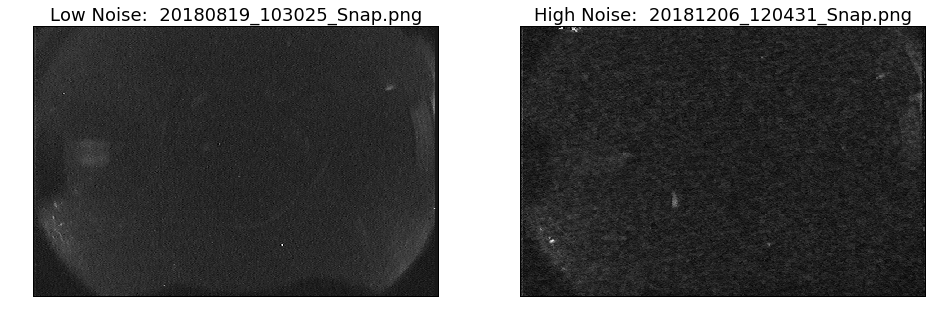
\includegraphics[width=1.2\textwidth]{images/low_and_high_noise.png}}
  \caption[A low noise D6 snapshot taken in August 2018 (left) alongside a high noise D6 snapshot taken in December 2018 (right).]{A low noise D6 snapshot taken in August 2018 (left) alongside a high noise D6 snapshot taken in December 2018 (right).  Noisy pixels provide issues for photometric analysis, which serves the foundation for fireball property estimates.}  
  \label{camera_noise}
\end{figure}

Not only was the camera noise problematic for photometric analysis, but it also made star recognition more difficult.
In many D6 snapshots, we were unable to recognize any celestial objects.
A lower-noise level could allow us to recognize more stars which would add to our star catalog, and increase the number of data points used to determine observable area.
There is also a chance that we could detect dimmer stars with less-noisy data, leading to a stronger understanding of our camera's capabilities.

\section{Outlook}

Moving forward, the most important thing to focus on is data collection.
Once the problem with unusually high volumes of systematic noise is dealt with, we will have most of the framework established to create a running fireball catalog.
However, we will need to create a script that estimates a fireball's properties (energy, mass, size) given the photometry program's outputted light curve.
This project however should be fairly straightforward and will utilize the equations such as Eq. \ref{area_eq} in the background chapter.

While a singular camera can serve an important role in fireball research, systems with multiple cameras stationed in different locations have certain benefits.
They allow for the triangulation of a given fireball which can then lead to more accurate velocity and position estimates.
With multiple systems, we could also estimate a fireball's orbital elements, and thus determine from whence it originated.
If we come to the conclusion that the D6 AllSky Camera is a feasible alternative in fireball research, we hope to construct another D6 AllSky camera that will lead to more precise data collection. 
The prospect of a secondary system is exciting and will hopefully help prove that the D6 AllSky camera is a desirable alternative in fireball research.